\documentclass[12pt]{article}
\usepackage{array}
\usepackage{amsmath}
\usepackage{amssymb}
\usepackage{algorithm}
\usepackage{algorithmic}
\usepackage{caption}
\usepackage{fontspec}
\usepackage{graphicx}
\usepackage{indentfirst}
\usepackage{minted}
\usepackage{mathtools}
\usepackage{pifont}
\usepackage{setspace}
\usepackage{subfigure}
\usepackage{tikz}
\usepackage{url}
\usepackage{xcolor}
\usepackage{xeCJK}

\usepackage[colorlinks=true]{hyperref}
\usepackage[margin=0.55in]{geometry}

% background color for minted
\definecolor{bg}{rgb}{0.95,0.95,0.95}

% CJK font
\setCJKmainfont{Source Han Serif CN}

% indent value
\setlength{\parindent}{2em}

% line spacing
\linespread{1.2}

\title{The Pixel Coordinates of a 3D Point}
\author{Yiteng Zhang}
%\date{}

\begin{document}
\maketitle

\indent{}如何找到三维点在二维像素坐标系下的位置是一个十分基础但又重要的问题,这对于光栅化渲染技术
而言是一个重要过程(另一个重要过程是Shading)。这里对Scratchapixel上的相关内容做了一些简单的整理和总
结,方便回顾。

\indent{}广义上的栅格化(Rasterisation)指的是将三维形状转变至栅格图像的过程。这里我们仍然可以用栅格化
来指代寻找三维中的点在二维像素坐标系中的位置这一过程。常用的渲染技术包括光栅化渲染和
光线追踪(Ray Tracing),虽然技术本质不同,但它们都依赖于\textbf{透视投影}这一基础概念的相关原理。

\indent{}透视投影的工作方式和人眼比较像,因而是从三维场景产生二维图像的自然方式。简单来说,可以通过将
三维空间中的点投影在画布(Canvas)所在的平面上,来得到其在二维中的表达。透视投影在视觉上的重要性质
是“近大远小”,这种效应被称为foreshortening。透视投影的过程非常简单,它基于三角形相似的几何原理。

\begin{figure}[h]
\centering
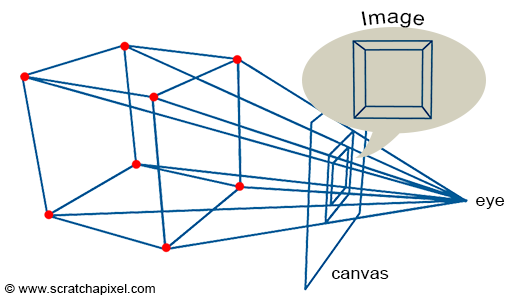
\includegraphics[width=9cm]{./imgs/perspective4.png}
\end{figure}

\indent{}在透视投影中,有一些重要的概念需要注意。“眼”的位置处于画布中心。画布的的尺寸是可变的,通过改
变其尺寸,可以进而改变视锥(Viewing Frustum)。所谓的视锥是这样定义的,我们从画布的每个角点发出射向眼
的线,再将这些线沿着另一方向延伸至场景中(直到眼能看到的距离为止),所形成的金字塔形的空间即为视锥,视锥
越大,眼能看到的场景就越多。可以看到,这种效果和改变相机镜头的焦距是一样的。改变画布大小,意味着我们改变
了视场(field of view,fov)。

\indent{}当一个点首次被定义于场景中时,我们就说它的坐标被定义在\textbf{世界空间}中:该点的坐标是相对于全
局或世界笛卡尔坐标系定义的。这个坐标系的原点被称之为\textbf{世界原点}。定义在世界空间中的点,其坐标是相对
于世界原点的。

\indent{}我们知道,可以使用平移(translation),旋转(rotation)与尺度(scale)操作对三维空间中的对象进行
变换。一个线性变换(即这三种操作的任意组合)可以被表示为一个$4\times 4$的矩阵$\mathbf{M}$。如果给定某一对
象上的变换矩阵$\mathbf{M}$,我们就可以知道该对象的姿态,或者说其在空间中的状态。至于为何是$4\times 4$
矩阵,如果参考\textbf{齐次坐标系}的定义,就会发现使用这种表达形式是很有好处的。

\begin{displaymath}
\mathbf{M} = \begin{bmatrix}
\color{red}{c_{00}}& \color{red}{c_{01}}&\color{red}{c_{02}}&\color{black}{c_{03}}\\
\color{green}{c_{10}}& \color{green}{c_{11}}&\color{green}{c_{12}}&\color{black}{c_{13}}\\
\color{blue}{c_{20}}& \color{blue}{c_{21}}&\color{blue}{c_{22}}&\color{black}{c_{23}}\\
\color{purple}{c_{30}}& \color{purple}{c_{31}}&\color{purple}{c_{32}}&\color{black}{c_{33}}\\
\end{bmatrix}
\begin{array}{l}
\rightarrow \quad \color{red} {x-axis}\\
\rightarrow \quad \color{green} {y-axis}\\
\rightarrow \quad \color{blue} {z-axis}\\
\rightarrow \quad \color{purple} {translation}\\
\end{array}
\end{displaymath}

\indent{}上式我们使用\textbf{行主序约定(row-major order convention)},那么矩阵对角线上的前三个系数$c_{00}$,$c_{11}$
和$c_{22}$编码了尺度操作。最后一行的前三个系数$c_{30}$,$c_{31}$和$_{32}$编码了平移操作。整个左上角的$3\times 3$
矩阵编码了旋转操作。那么,我们可以将对应操作拆解为:

\begin{displaymath}
\mathbf{R} =
\begin{bmatrix}
\color{red}{c_{00}}& \color{red}{c_{01}}&\color{red}{c_{02}}\\
\color{green}{c_{10}}& \color{green}{c_{11}}&\color{green}{c_{12}}\\
\color{blue}{c_{20}}& \color{blue}{c_{21}}&\color{blue}{c_{22}}\\
\end{bmatrix} \quad\quad
\mathbf{t} = \begin{bmatrix}
\color{purple}{c_{30}}& \color{purple}{c_{31}}&\color{purple}{c_{32}}
\end{bmatrix}
\end{displaymath}

\indent{}当我们定义了世界坐标系之后,我们就可以创建其他的笛卡尔坐标系。与点的定义相同,这些新的坐标系由其在世
界空间中的位置来定义,也同样有三个彼此正交的单位向量作为轴。新的坐标系的位置可以表达为translation的值,其三个
主轴也由世界坐标系中的向量来表示,这对应于$\mathbf{M}$左上角的$3\times 3$矩阵。一个$4\times 4$矩阵可以用来描述
一个新的坐标系,它的定义是相对于世界坐标系的:

\begin{itemize}
\item 第一行的$(\color{red}{c_{00}}, \color{red}{c_{01}}, {\color{red}{c_{02}}})$对应于新坐标系的$x$轴,即
其$x$轴上的单位向量在世界坐标系下的表达;
\item 第二行的$(\color{green}{c_{10}}, \color{green}{c_{11}}, {\color{green}{c_{12}}})$对应于新坐标系
的$y$轴,即其$y$轴上的单位向量在世界坐标系下的表达;
\item 第三行的$(\color{blue}{c_{20}}, \color{blue}{c_{21}}, {\color{blue}{c_{22}}})$对应于新坐标系
的$z$轴,即其$z$轴上的单位向量在世界坐标系下的表达;
\item 第四行的$(\color{purple}{c_{30}}, \color{purple}{c_{31}}, {\color{purple}{c_{32}}})$对应于新坐标
系的位置,即其原点(origin)在世界坐标系下的表达。
\end{itemize}

\begin{figure}[h]
\centering
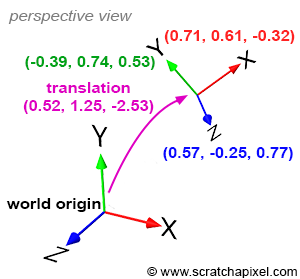
\includegraphics[width=5cm]{./imgs/coordsys.png}
\end{figure}

\noindent{}举例来说,与上图中的新坐标系对应的变换矩阵可以表示为:

\begin{displaymath}
\begin{bmatrix}
\color{red}{+0.71}&\color{red}{+0.61}&\color{red}{-0.32}&0\\
\color{green}{-0.39}&\color{green}{+0.74}&\color{green}{+0.53}&0\\
\color{blue}{+0.57}&\color{blue}{-0.25}&\color{blue}{+0.77}&0\\
\color{purple}{+0.52}&\color{purple}{+1.25}&\color{purple}{-2.53}&1\\
\end{bmatrix}
\end{displaymath}

\indent{}总而言之,我们可以说一个$4\times 4$矩阵实际上表示了一个坐标系,该局部坐标系(local system)的表示是相对于某个
全局坐标系的(global system),全局坐标系往往是世界坐标系。

\indent{}对于场景中的某个点,其坐标可以是相对于任意坐标系的。一个点的坐标可以有不同的表达,但这些表达都
表示着同一个点,只是参考系不同罢了。在实践中,使用相对于local坐标系的表达往往会更加方便,在必要时,我们可以做表达
的转换,将某个点在一个坐标系下的表达换到另一个坐标系下。

\begin{figure}[h]
\centering
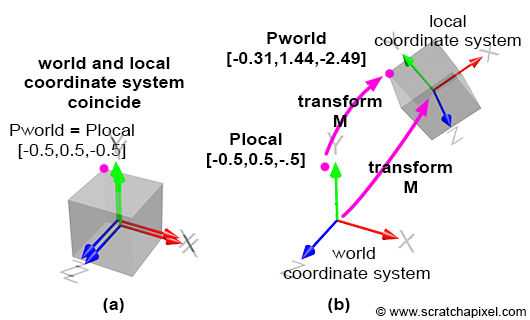
\includegraphics[width=8cm]{./imgs/coordsys2.png}
\end{figure}

\indent{}为了能够将点的表达在不同的坐标系下进行转换,我们需要的是local-to-world matrix与world-to-local matrix这两
类矩阵,分别将某一局部坐标系中的点的表达转换到世界坐标系下,将相对于世界坐标系的点的表达转换到某个局部坐标系
下。就 local-to-world 而言,我们之所以这么称呼,是因为 local 坐标系是相对于世界坐标系定义的,因而有:
\begin{align*}
&P_{world} = P_{local} * \mathbf{M}\\
&P_{local} = P_{world} * \mathbf{M}^{-1}
\end{align*}
\noindent{}之前定义的$4\times 4$矩阵$\mathbf{M}$即为 local-to-world matrix 在这里的表达。

\indent{}如果我们打算将三维场景投影至二维,相机是必不可少的。实际上,相机和其他的三维空间中的对象没有什么不
同,只不过我们用它来拍摄图像。使用相机时,我们需要移动和旋转相机来调整视角。在这种意义上,我们其实是在对相
机做transformation,即 translating 和 rotating 相机。我们真正在做的事情,是在变换一个局部坐标系,这个局部坐标
系是相机相对于世界坐标系的表达,我们称之为\textbf{相机坐标系(camera coordinate system)}。一个需要注意的地方
是,在习惯上,相机坐标系的 $z$ 轴向内指向相机屏幕(screen)。

\begin{figure}[h]
\centering
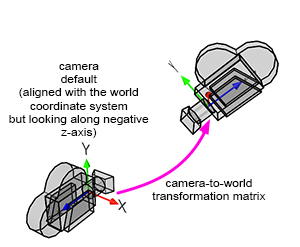
\includegraphics[width=6cm]{./imgs/camera2.png}
\end{figure}

\indent{}我们将前述的坐标系变换规则应用到这里,就可以知道定义在世界空间中的点在相机坐标系下的表达了,这可以
通过一个类似于 world-to-local 的转换得到。一旦将三维空间中的对象的表达都转换为相对于相机的,就可以在
同一 local 坐标系(即相机坐标系)下进行透视投影。

\indent{}至此,我们已经准备好将三维空间中的点向二维投影(具体来说,是向 screen space 投影)。我们将会把三维
点投影至画布(canvas)上,画布是一个二维面,我们在其上绘制三维场景。

\begin{figure}[h]
\centering
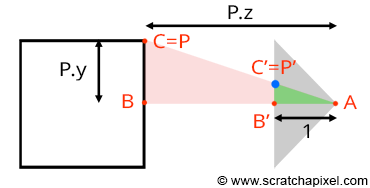
\includegraphics[width=6cm]{./imgs/box-setup4.png}
\end{figure}

\indent{}通过透视投影,我们将三维点投影到画布上,画布所在平面被称为投影平面或者像平面。如果我们追踪从 P 点
到眼的线(眼在这里即是相机坐标系原点),那么 $P'$ 是这条线和画布的交点。考虑 $\triangle ABC$ 和
$\triangle AB'C'$,根据相似三角形关系,可知:

\begin{displaymath}
\frac{BC}{AB} = \frac{B'C'}{AB'}
\end{displaymath}

\noindent{}如果屏幕到相机中心的距离是单位距离,那么在相机坐标系下,可知

\begin{displaymath}
\frac{P.y}{P.z} = \frac{P'.y}{1} \;\;\Rightarrow \;\; P'.y = \frac{P.y}{P.z}
\end{displaymath}

\noindent{}这个关系是计算机图形学中最为基础的关系之一,它被称为 perspective-divide 或 z-divide,这对
于 $x$ 方向也是成立的,即投影点的 $x$ 方向的坐标 $x'$ 是

\begin{displaymath}
P'.x = \frac{P.x}{P.z}
\end{displaymath}

\noindent{}总结一下,将一个定义在世界坐标系下的三维点投影至画布的过程为:
\begin{enumerate}
\item $P_{camera} = P_{world} * M_{world-to-camera}$
\item $P'.x = \dfrac{P_{camera}.x}{P_{camera}.z}, \;\; P'.y = \dfrac{P_{camera}.y}{P_{camera}.z}$
\end{enumerate}

\noindent{}注意,因为相机坐标系的 $z$ 轴是向内的,只有相机空间中的点的 $z$ 坐标为负时,该点才是可见的。

\indent{}到目前为止,我们已经知道如何将点投影到画布上,但我们最终想知道的是它在像素坐标系(栅格坐标系)中
的位置,所以还有一系列过程要进行,将涉及到三个坐标系:屏幕坐标系(screen coordinate system),标准
化设备坐标系(NDC coordinate system)和栅格坐标系(raster coordinate system)。

\begin{figure}[h]
\centering
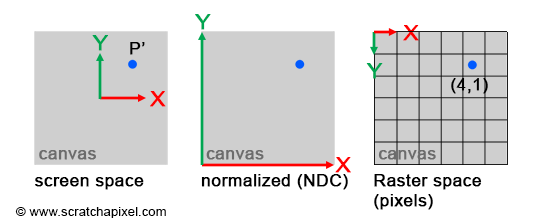
\includegraphics[width=9cm]{./imgs/screen_ndc_raster.png}
\end{figure}

\indent{}投影至画布上的点$P'$ 是定义在投影平面上的。投影平面是一个几何平面,是无限大的,然而图像或屏幕的尺寸
是有限的,具有一个有限的宽度和高度。因此投影至像平面(即投影平面)的点并不一定都是最终可见的,我们需要舍弃屏
幕外的区域。或者说,我们会从投影平面上切下一个以图像中心为中心点的矩形区域,这对应于屏幕坐标系。

\begin{figure}[h]
\centering
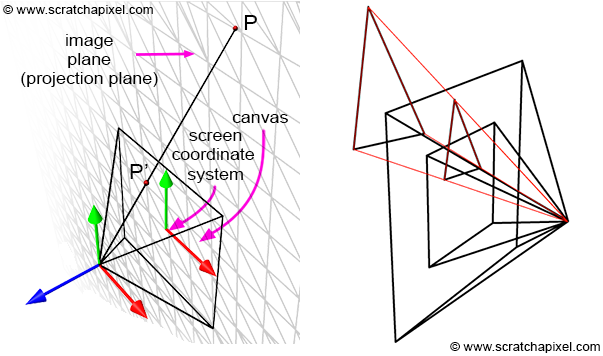
\includegraphics[width=8cm]{./imgs/screen.png}
\end{figure}

\indent{}当然,改变画布的大小会影响可见区域的范围。如前所述,画布大小和 fov 是互相相关的。如果我们有一个宽为 $w$,高
为$h$的画布,那么可见性区域应该满足:
\begin{displaymath}
|P'.x| \leqslant \frac{w}{2}, \;\; |P'.y| \leqslant \frac{h}{2}
\end{displaymath}

\indent{}一个关键的问题是,screen space 中的点的坐标是实数,是定义在连续空间上的。然而,数字图像是用像素表达
的,其上的点的坐标是整数,是离散的,以像素为单位。其坐标的原点位于图像的左上角,$x$ 轴指向右侧,$y$ 轴指向下方,这
种坐标系被称为栅格坐标系。我们真正想要得到的是三维点在栅格坐标系中的位置。

\indent{}现在,我们需要进行从 screen space 转到 NDC space,再转到 raster space 的过程。首先,我们需要将 $P'$ 的坐
标值重映射至 $[0,1]\in \mathbb{R}$,也就是做归一化。具体来说,需要进行下述映射:

\begin{displaymath}
\begin{array}{l}
P'_{normalized}.x = \dfrac{P'.x + w / 2}{ w }\\
P'_{normalised}.y = \dfrac{P'.y + h / 2}{ h }
\end{array}
\end{displaymath}

\noindent{}得到的新的坐标即是定义在 NDC space 中的值。标准化设备坐标系(NDC coordinate system)的原点位于画布
的左下角位置,该坐标系中的点的坐标取值都在区间 $[0,1]\in \mathbb{R}$ 中。

\indent{}最后一步,我们将把点在 NDC space 中的坐标转换至像素空间(也就是 raster space)中,即从 NDC 坐标系下
的表达转换至 raster 坐标系下的表达。我们知道,图像是以像素为单位的。假设我们拍摄得到的图像宽 $W$ 个像
素,高 $H$ 个像素,我们需要将坐标值从区间 $[0,1]\in \mathbb{R}$ 映射到 $[0, W]\in \mathbb{N}$ 或
$[0, H]\in \mathbb{N}$ 上。对于 NDC 坐标系下的点 $P'_{normalized}$,通过下述过程将其转换为栅格
坐标系下的表达:

\begin{displaymath}
\begin{array}{l}
P'_{raster}.x = \lfloor{ P'_{normalized}.x * W}\rfloor\\
P'_{raster}.y = \lfloor{ (1 - P'_{normalized}.y) * H}\rfloor
\end{array}
\end{displaymath}
\noindent{}上面的映射过程中,需要注意栅格坐标系的 $y$ 轴是向下的,与 NDC 坐标系的 $y$ 轴方向相反。

\indent{}到这里,整个流程就结束了,我们一步步地找到了三维空间中的一个点在对应二维图像中的位置。在这个
流程中,我们一次次地寻找一个点在不同空间中的表达:

\begin{displaymath}
\text{World Space} \rightarrow \text{Camera Space} \rightarrow \text{Screen Space}
\rightarrow \text{NDC Space} \rightarrow \text{Raster Space}.
\end{displaymath}

\noindent{}最终确定了所要寻找的点对应于哪个位置的像素。

\end{document}